\section{Data preparation}
\label{sec:data_preparation}

To successfully train FESD three steps are taken before training can begin, data augmentation, data merging, and data balancing. The data augmentation is done to ensure that the model is robust to different variations in the data. The data merging is done to combine the different modalities into a single tensor. The data balancing is done to ensure that the model is not biased toward any particular error label.

The finished data preparation pipeline can be seen in Figure \ref{fig:data_preparation_pipeline}.

\begin{figure}
  \centering
  \includegraphics[width=\linewidth]{figures/Model/Data_Preparation_Pipeline.png}
  \caption[Data preparation pipeline]{The data preparation pipeline. The data is first augmented, then merged, and finally balanced.}
  \label{fig:data_preparation_pipeline}
\end{figure}

The images that are stored by \textit{FESDData} are inherently the same size. The joints, however, are stored within a JSON file containing the coordinates of each joint in 2D and 3D. To further process the 2D joint data is drawn on an image that
 has the same dimensions as the RGB and Depth image.

\subsection{Data augmentation}

Four different augmentations are applied to the data to generalise the data. The first augmentation is flipping the data. The RGB image, the depth image, and the joint image are flipped horizontally. Furthermore, the ground truth data is flipped, as labels refer to the left or right side of the body, which would no longer coincide with the data that is passed into the network.

Additionally, the images are cropped at random while keeping the positions of the joints and a margin around the joints visible. This ensures that the model is robust to different positions of the user in the image. 

Finally, at random Gaussian noise is applied to the RGB image and the depth image. This further improves the robustness of irregular data.

The augmentations can be seen in Figure \ref{fig:data_preparation_pipeline} where they are applied to a sample frame from the dataset.

\subsection{Data merging}

While there are different ways of applying transfer learning to the problem at hand, we chose to merge the different modalities into a single tensor. This allows us to use the EfficientNet v2 as a feature extractor for all modalities, without the added computations of extracting the features of each modality individually. The data is merged by assigning each modality to a channel in an RGB image.

In Figure \ref{fig:data_preparation_pipeline} we can see the different modalities as they are merged into a single tensor. The RGB image is transformed into greyscale and assigned to the red channel, the depth image is scaled to a value between 0 and 255 and assigned to the green channel, and the joint coordinates are assigned to the blue channel. The data is then passed into the EfficientNet v2 as a single RGB image.

\subsection{Data balancing}

In the ordinary case, human pose estimation is not meant to produce faulty results. In the selected exercises it is aimed to produce faulty results. However, this does still not produce a balanced dataset. In section \ref{sec:dataset}, the statistics of the dataset are shown. Especially, in Figure \ref{fig:err_dist_joint_pie, fig:err_dist_limb_pie, fig:err_dist_half_pie, fig:err_dist_full_pie} it can be seen that the dataset is imbalanced. Most notably for the problem set \textit{Half} and \textit{Full} where the error label \textit{No Error} is overrepresented.

To balance the dataset, frames are sampled using a Weighted Random Sampler for each batch of the training. The weights for the samples are calculated based on the occurrence of the error labels in the dataset. While only considering the whole body as a single object, the calculation of the weights is simple. For each frame, the error label is counted and the inverse of the count is used as the weight for the frame. This ensures that the model is not biased toward any particular error label by oversampling the frames which contain an error.

However, for the other problem sets the calculation of the weights is more complex. In the other problem sets each frame contains an error for each area, e.g. when considering the Half-Body problem, the upper and lower body 2 errors. To successfully balance the dataset for each area four weights would need to be created and balanced, i.e. the upper and lower body have an error the upper body is faulty and the lower body is not, etc. This would oversample some frames while undersampling others. In the other problem sets this is far more visible. Therefore, it was decided to consider the sum of errors is considered as a single error label. This means that frames that have the same number of erroneous areas are weighed the same.

An example of the distribution of errors before and after balancing can be seen in Figure \ref{fig:balance} for each problem set.

% In previous sections, we have explained the structure of the data and how the data is labeled. In this section, we will explain how the data is prepared for training. The data preparation consists of two parts, data augmentation, and data splitting.

% After the data has been split and augmented, the data is stored in tensors of a fixed size. If an image is too small we apply a bilinear interpolation to resize the image. If an image is too large we crop the side. The images are resized to $300 \times 300$ pixels.

% \subsection{Data augmentation}
% \label{sec:data_augmentation}

% To ensure that the model is robust to different variations in the data, the data is augmented. We apply three different forms of augmentation to the data. The first form of augmentation is flipping the data. The RGB image, the depth image, and the relative joint coordinates are flipped horizontally. Furthermore, we apply random and non-random cropping to the visual data. We ensure that none of the joints are outside the image. We also apply random padding when the image is cropped. The final augmentation is Gaussian noise. We apply Gaussian noise to the RGB image and the depth image. In Figure \ref{fig:augmentation} we can see the different augmentations.

% \begin{figure}
%     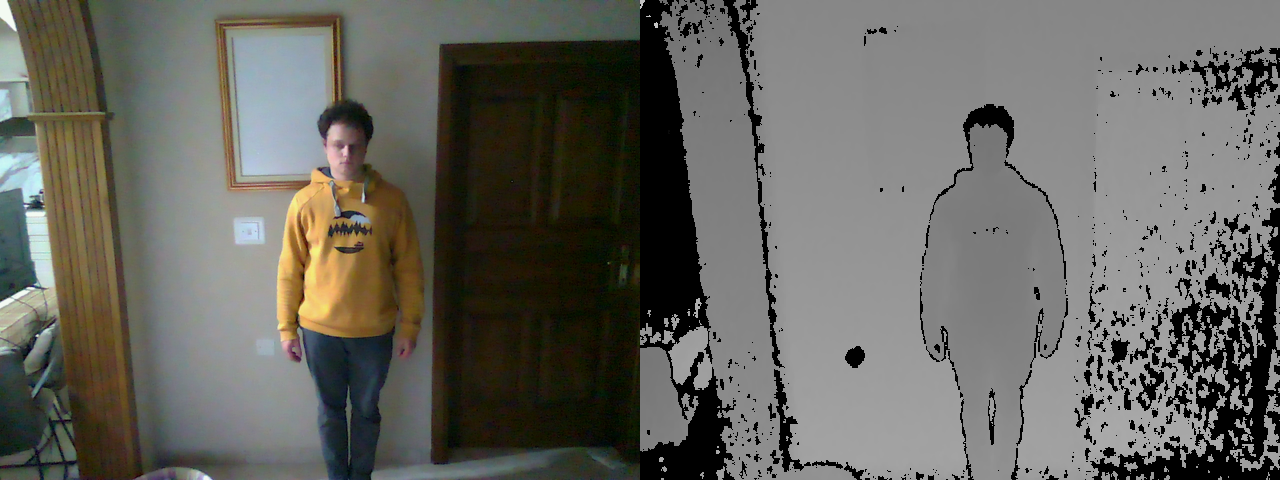
\includegraphics[width=.33\textwidth]{figures/Model/Augmentation/Original.png}\hfill
%     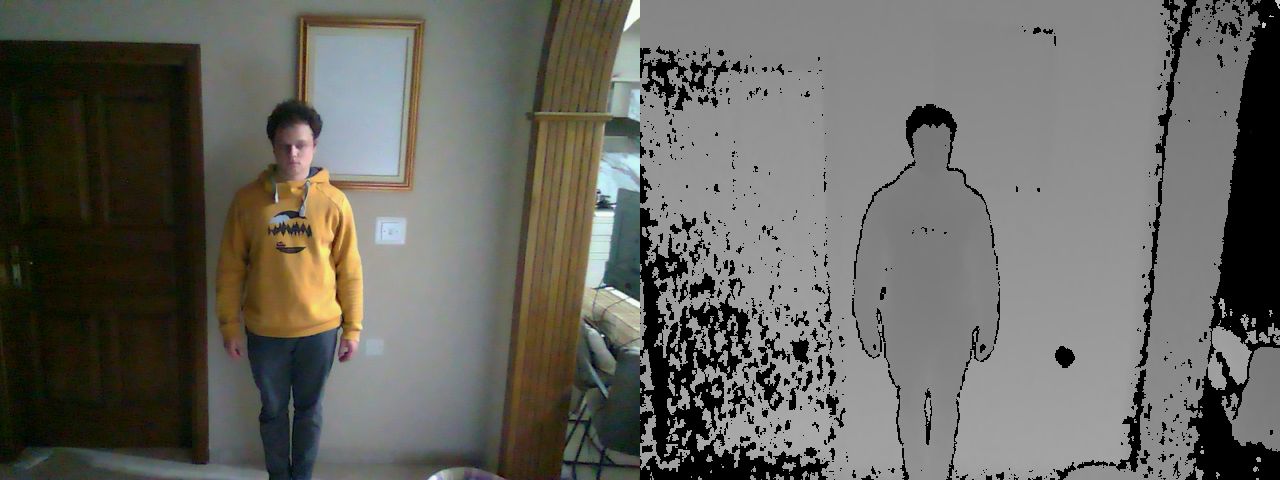
\includegraphics[width=.33\textwidth]{figures/Model/Augmentation/Flipped.png}\hfill
%     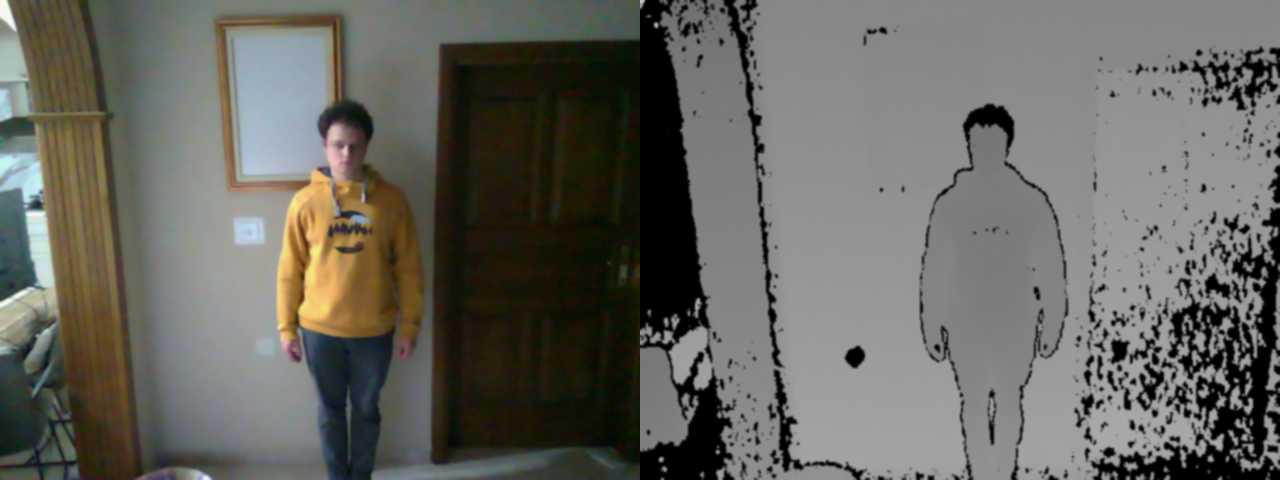
\includegraphics[width=.33\textwidth]{figures/Model/Augmentation/GaussianBlur.png}
%     \\[\smallskipamount]
%     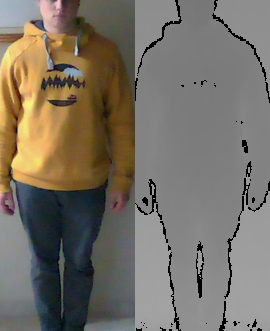
\includegraphics[width=.33\textwidth]{figures/Model/Augmentation/Cropped.png}\hfill
%     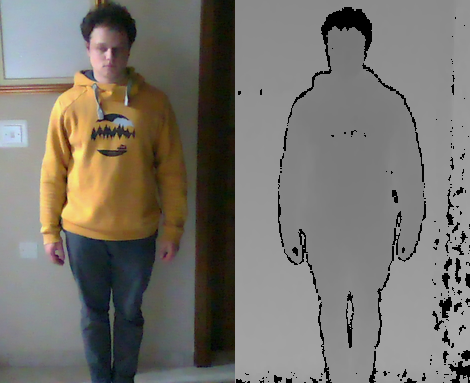
\includegraphics[width=.33\textwidth]{figures/Model/Augmentation/CroppedPad50.png}\hfill
%     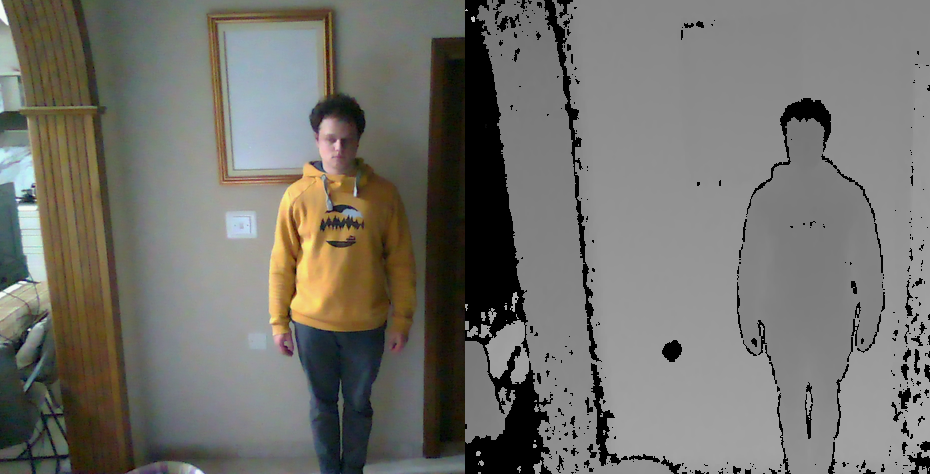
\includegraphics[width=.33\textwidth]{figures/Model/Augmentation/RandomCropped.png}
%     \caption[Data Augmentation]{Augmentation applied to a sample frame. The augmentations are; Horizontal flipping, Gaussian Blur, Exact Cropping, Exact Cropping with padding, and random Cropping respectively.}\label{fig:augmentation}
% \end{figure}


% \subsection{Data splitting}

% The data is split into two parts. The first part is the training data. The training data is used to train the model. To test the validity of the model itself, we split the data by exercise. We define 4 exercises, which are not used during training. We chose the exercises such that each exercise is in a different difficulty category, i.e. one of the exercises for testing has a trivial difficulty, one is considered as easy, and so on. With this, we try to find if our model performs better or worse with increased difficulty on unseen data.
